\section{Supervised Fine-Tuning for Sparse Reasoning and Cross-Context Memory}
\label{sec:sft}

CPT learns transferable action control from visual observations, while supervised fine-tuning (SFT) teaches the model to follow explicit task objectives. We train on tasks at different difficulty levels, from local operations and intermediate subgoals to complete objectives, with reasoning and memory summaries at key decision points. The need for reasoning is inherently sparse in long-horizon gameplay. Routine movement and repeated attacks favor direct action, while route failures, target switches, and resource decisions often require replanning. \ourmodel therefore uses a single autoregressive policy to alternate between direct control, sparse reasoning, and memory updates. Persistent summaries carry task state across context boundaries. Figure~\ref{fig:sft_overview} illustrates how adaptive reasoning and memory compaction are integrated into an interaction sequence.


\begin{figure}[H]
    \centering
    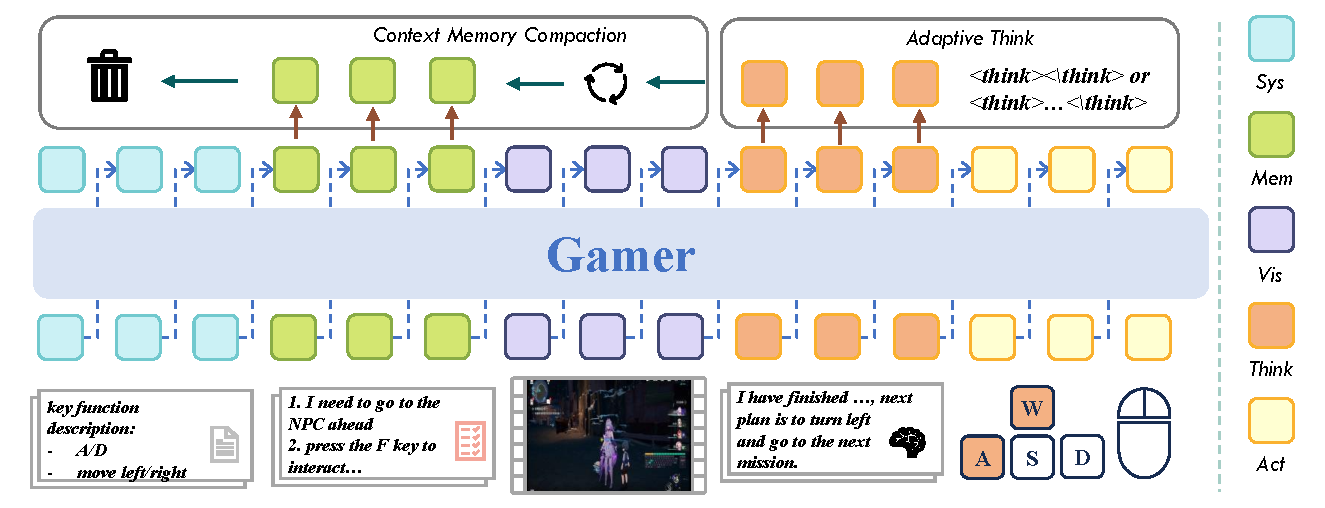
\includegraphics[width=0.94\linewidth]{figs/sft.pdf}
    \caption{
    \textbf{Sparse reasoning and cross-context memory in supervised fine-tuning.}
    The shared autoregressive policy integrates visual observations, task memory, optional reasoning, and executable keyboard-mouse actions. Context memory compaction preserves task progress across long interactions, while adaptive reasoning allows the policy to act directly at routine steps and generate explicit reasoning when needed.
    }
    \label{fig:sft_overview}
\end{figure}


\subsection{Multi-level Task Conditioning and Sparse Reasoning}
\label{sec:sparse_reasoning}

SFT retains the control specification $\mathcal{B}$ and recent interaction history $\mathcal{H}_t$ introduced during CPT, and additionally conditions the policy on a task instruction $I$ and long-term memory $\mathcal{M}_t$. The resulting context is
\[
(\mathcal{B}, I, \mathcal{M}_t, \mathcal{H}_t),
\]
where $\mathcal{H}_t$ contains the current observation together with recent observations, actions, and previously generated reasoning. To expose the policy to task structure at different temporal scales, the instruction $I$ is instantiated at three difficulty levels:
\[
I
\in
\left\{
I^{\mathrm{op}},
I^{\mathrm{sub}},
I^{\mathrm{task}}
\right\},
\]
in which $I^{\mathrm{op}}$, $I^{\mathrm{sub}}$, and $I^{\mathrm{task}}$ correspond to local operations, intermediate subgoals, and complete tasks, respectively. Training data at all three levels use the same observation–action interface and are used to train a single policy that produces executable keyboard and mouse actions.

At each interaction step, the model first generates an optional reasoning sequence $r_t$ and then produces the executable action $a_t$. Their joint distribution follows the autoregressive generation order:
\begin{equation}
\pi_\theta
\left(
r_t,a_t
\mid
\mathcal{B},I,\mathcal{M}_t,\mathcal{H}_t
\right)
=
\pi_\theta
\left(
r_t
\mid
\mathcal{B},I,\mathcal{M}_t,\mathcal{H}_t
\right)\cdot
\pi_\theta
\left(
a_t
\mid
\mathcal{B},I,\mathcal{M}_t,\mathcal{H}_t,r_t
\right).
\label{eq:sft_joint_policy}
\end{equation}

The reasoning sequence takes one of three forms:
\begin{equation}
r_t
\in
\left\{
\varnothing,
r_t^{\mathrm{cur}},
r_t^{\mathrm{mem}}
\right\},
\label{eq:reasoning_types}
\end{equation}
when $r_t = \emptyset$, $\pi_\theta(a_t \mid \mathcal{B}, I, \mathcal{M}_t, \mathcal{H}_t, r_t)$ naturally simplifies to $\pi_\theta(a_t \mid \mathcal{B}, I, \mathcal{M}_t, \mathcal{H}_t)$.
$r_t^{\mathrm{cur}}$ denotes reasoning for the current decision and $r_t^{\mathrm{mem}}$ denotes a memory summary for future contexts. At routine control steps, the model sets $r_t=\varnothing$ and generates an action directly. At decision-critical or memory-update steps, the model generates reasoning before the action. Current reasoning captures immediate judgment, next subgoal, or short-term plan, such as revising a route, selecting an interaction target, or switching combat strategy. Memory summaries, by contrast, retain information needed beyond the current context, including task progress, important locations, resource states, failed attempts, and remaining plans. The policy learns when to generate reasoning within the same autoregressive process, without a separate classifier or routing head. Here, $r_t$ refers only to the explicitly supervised reasoning text generated by the policy and does not characterize all latent computation within the model.

SFT trains current reasoning, memory summaries, and executable actions within the same autoregressive output space. Let
\[
y_t=[r_t,a_t]
\]
denote the complete output sequence at step $t$, and let $y_{t,<j}$ denote the generated prefix before its $j$-th token. The SFT objective is
\begin{equation}
\mathcal{L}_{\mathrm{SFT}}
=
-
\sum_t
\sum_{j=1}^{|y_t|}
\log
\pi_\theta
\left(
y_{t,j}
\mid
\mathcal{B},
I,
\mathcal{M}_t,
\mathcal{H}_t,
y_{t,<j}
\right).
\label{eq:sft_objective}
\end{equation}

The objective uses the same token-level autoregressive formulation as CPT, with the target extended from the action $a_t$ to the reasoning-action sequence $[r_t,a_t]$. It also introduces the task instruction $I$ and long-term memory $M_t$ into the conditioning context.

\subsection{Summary-Based Cross-Context Memory}
\label{sec:cross_context_memory}


Long-horizon tasks require the agent to retain relevant information after earlier observations and actions leave the active context. We update long-term memory $\mathcal{M}_t$ when the task changes stage, a subgoal is completed, or older interactions are about to leave the active context. Consider a memory-update step in which the short-term history $\mathcal{H}_t$ is partitioned as
\[
\mathcal{H}_t
=
\mathcal{H}_t^{\mathrm{old}}
\oplus
\mathcal{H}_t^{\mathrm{keep}},
\]
where $\mathcal{H}_t^{\mathrm{old}}$ contains earlier interactions that will leave the active context, $\mathcal{H}_t^{\mathrm{keep}}$ contains recent interactions that remain directly accessible, and $\oplus$ denotes temporal concatenation.

Before $\mathcal{H}_t^{\mathrm{old}}$ is discarded, the model generates a memory summary from the complete information currently available. The long-term memory and short-term history are then updated as
\begin{equation}
r_t^{\mathrm{mem}}
\sim
\pi_\theta
\left(
\cdot
\mid
\mathcal{B},I,\mathcal{M}_t,\mathcal{H}_t
\right),
\qquad
\left(
\mathcal{M}_t^{+},
\mathcal{H}_t^{+}
\right)
=
\left(
\bar {\mathcal{M}_t}
\oplus
r_t^{\mathrm{mem}},
\mathcal{H}_t^{\mathrm{keep}}
\right).
\label{eq:memory_update}
\end{equation}

Here, $\mathcal{M}_t^{+}$ and $\mathcal{H}_t^{+}$ denote the updated long-term memory and short-term history. $\bar {\mathcal{M}_t}$ denotes the portion of the previous memory retained after reserving space for the new summary. When the memory budget is exceeded, the oldest complete summaries are removed in temporal order.

The update preserves overall task progress in memory and recent interaction details in the active history. Task-relevant information contained in $\mathcal{H}_t^{\mathrm{old}}$ is carried forward through $r_t^{\mathrm{mem}}$, while fine-grained recent evidence remains directly accessible in $\mathcal{H}_t^{\mathrm{keep}}$. When memory is updated at a task boundary without context eviction, we set $\mathcal{H}_t^{\mathrm{old}}=\varnothing$ and $\mathcal{H}_t^{\mathrm{keep}}=\mathcal{H}_t$.

A memory-update step remains an ordinary interaction step. After generating $r_t^{\mathrm{mem}}$, the policy still produces the corresponding executable action $a_t$. Memory generation remains part of the reasoning–action process, allowing closed-loop control to continue without help from another memory model. During training, each step uses only the information that would be available at inference time. Each memory summary is generated only from interactions available at the corresponding update point. Subsequent trajectory segments are conditioned on the updated memory together with the retained recent history. The policy thus learns to continue a task after parts of its interaction history are no longer directly accessible.
